\documentclass[unboxed]{hwset}

\usetikzlibrary{patterns}
\def\hexagonsize{0.6cm}
\pgfdeclarepatternformonly
  {hexagons}% name
  {\pgfpointorigin}% lower left
  {\pgfpoint{3*\hexagonsize}{0.866025*2*\hexagonsize}}%  upper right
  {\pgfpoint{3*\hexagonsize}{0.866025*2*\hexagonsize}}%  tile size
  {% shape description
  \pgfsetlinewidth{0.4pt}
  \pgftransformshift{\pgfpoint{0mm}{0.866025*\hexagonsize}}
  \pgfpathmoveto{\pgfpoint{0mm}{0mm}}
  \pgfpathlineto{\pgfpoint{0.5*\hexagonsize}{0mm}}
  \pgfpathlineto{\pgfpoint{\hexagonsize}{-0.866025*\hexagonsize}}
  \pgfpathlineto{\pgfpoint{2*\hexagonsize}{-0.866025*\hexagonsize}}
  \pgfpathlineto{\pgfpoint{2.5*\hexagonsize}{0mm}}
  \pgfpathlineto{\pgfpoint{3*\hexagonsize+0.2mm}{0mm}}
  \pgfpathmoveto{\pgfpoint{0.5*\hexagonsize}{0mm}}
  \pgfpathlineto{\pgfpoint{\hexagonsize}{0.866025*\hexagonsize}}
  \pgfpathlineto{\pgfpoint{2*\hexagonsize}{0.866025*\hexagonsize}}
  \pgfpathlineto{\pgfpoint{2.5*\hexagonsize}{0mm}}
  \pgfusepath{stroke}
}

\name{Erich L Foster}
\class{Calculus I}
\duedate{26 April 2011}
\assignment{Homework 12}

\begin{document}
\begin{problem}[1.]
  \tbf{Let's design a can.}
  \begin{enumerate}
    \item A can is to be made to hold volume V. Find the ratio between the
      height $h$ and the radius $r$ that will minimize the cost of the metal to
      manufacture the can, assuming the cost is directly proportional to the
      metal used.
    \item In part (a) we assumed there to be no waste in the making of the can.
      However, in manufacturing the can we must have some waste when creating
      the top and bottom discs. Now assume the top and bottom discs are cut from
      squares as in Figure \ref{fig:squares} and find the ratio of the height
      $h$ to the radius $r$ that minimizes the cost of manufacturing the can.
    \item A more efficient packing of discs can be obtained by diving the metal
      sheet into hexagons and cutting the discs from the hexagons as in Figure
      \ref{fig:hexagons}. If this strategy is adopted find the ratio between the
      height $h$ and the radius $r$ that minimizes the cost of manufacturing the
      can.
  \end{enumerate}
\end{problem}

  \begin{figure}[h]
    \begin{minipage}[b]{0.5\linewidth}
    \begin{center}
	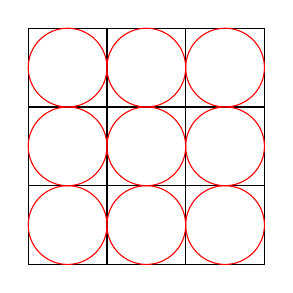
\begin{tikzpicture}[scale=0.5]
    \draw[black] (0,2) -- (6,2) -- (6,-4) -- (0,-4) -- cycle;
    \draw[black] (2,2) -- (2,-4);
    \draw[black] (4,2) -- (4,-4);
    \draw[black] (0,0) -- (6,0);
    \draw[black] (0,-2) -- (6,-2);
    \draw[red] (1,1) circle (1);
    \draw[red] (3,1) circle (1);
    \draw[red] (5,1) circle (1);
    \draw[red] (1,-1) circle (1);
    \draw[red] (3,-1) circle (1);
    \draw[red] (5,-1) circle (1);
    \draw[red] (1,-3) circle (1);
    \draw[red] (3,-3) circle (1);
    \draw[red] (5,-3) circle (1);
	\end{tikzpicture}
    \end{center}
    \caption{Discs cut from squares}
    \label{fig:squares}
    \end{minipage}
    \hspace{0.5cm}
    \begin{minipage}[b]{0.5\linewidth}
    \begin{center}
	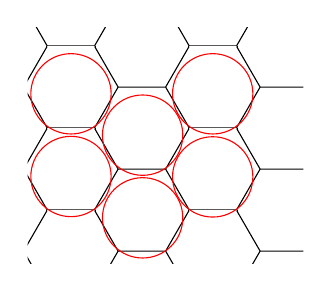
\begin{tikzpicture}[scale=0.5]
    \fill[pattern=hexagons] (-2,2) rectangle (5,-4);

    \draw[red] (-0.9,0.32) circle (1.02);
    \draw[red] (-0.9,-1.78) circle (1.02);
    \draw[red] (0.92,-0.73) circle (1.02);
    \draw[red] (0.92,-2.83) circle (1.02);
    \draw[red] (2.7,0.32) circle (1.02);
    \draw[red] (2.7,-1.79) circle (1.02);
	\end{tikzpicture}
    \end{center}
    \caption{Discs cut from squares}
    \label{fig:hexagons}
    \end{minipage}
  \end{figure}

\begin{problem}[2.]
  Show that the rectangle with the largest area inscribed in a circle is a
  square.
\end{problem}

\begin{problem}[3.]
  Show that if $x,y,\text{ and } z$ are positive numbers then
  \begin{equation*}
    \dfrac{\left( x^2 + 1 \right)\left( y^2 + 1 \right)\left( z^2 + 1
    \right)}{xyz} \ge 8
  \end{equation*}
  Hint: If $A$ and $B$ are both minimal then so is $AB$.
\end{problem}

\end{document}
